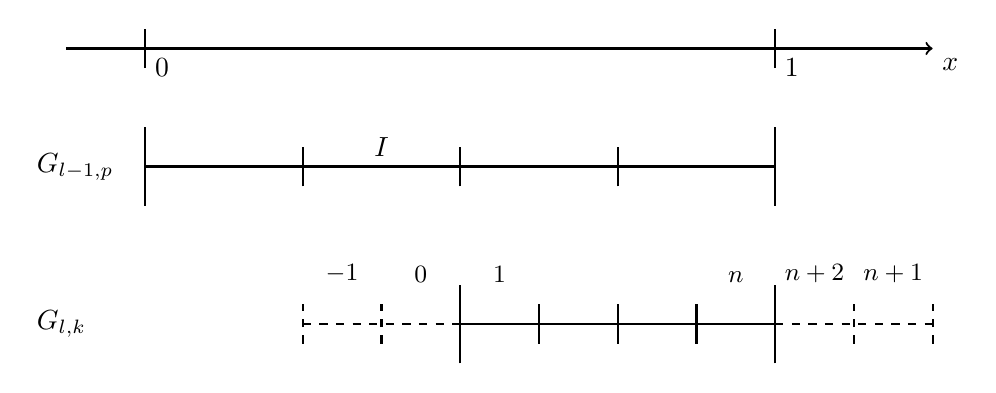
\begin{tikzpicture}

    % axe des abscisses
    \draw[->, thick] (-1, 3.5) -- (10,3.5);
    \draw[thick] (0, 3.25) -- (0, 3.75);
    \draw[thick] (8, 3.25) -- (8, 3.75);

    \node[below right] at (10, 3.5) {\( x \)};
    \node[below right] at (0, 3.5) {\( 0 \)};
    \node[below right] at (8, 3.5) {\( 1 \)};

    
    % maillage parent
    
    % ligne horizontale
    \draw[thick] (0, 2) -- (8, 2);

    % lignes verticales
    \draw[thick] (0, 1.5) -- (0, 2.5);
    \draw[thick] (8, 1.5) -- (8, 2.5);
    \draw[thick] (2, 1.75) -- (2, 2.25);
    \draw[thick] (4, 1.75) -- (4, 2.25);
    \draw[thick] (6, 1.75) -- (6, 2.25);

    % Annotations
    \node[right] at (-1.5, 2) {\(G_{l-1, p}\)};
    \node[above] at (3, 2) {\(I\)};

    % maillage secondaire

    % ligne horizontale    
    \draw[thick] (4, 0) -- (8, 0);

    % lignes verticales
    \draw[thick] (4, -0.5) -- (4, 0.5);
    \draw[thick] (8, -0.5) -- (8, 0.5);
    \draw[thick] (5, -0.25) -- (5, 0.25);
    \draw[thick] (6, -0.25) -- (6, 0.25);
    \draw[thick] (7, -0.25) -- (7, 0.25);

    % Mailles fantômes
    \draw[dashed, thick] (2, 0) -- (4, 0);
    \draw[dashed, thick] (8, 0) -- (10, 0);
    \draw[dashed, thick] (2, -0.25) -- (2, 0.25);
    \draw[dashed, thick] (3, -0.25) -- (3, 0.25);
    \draw[dashed, thick] (9, -0.25) -- (9, 0.25);
    \draw[dashed, thick] (10, -0.25) -- (10, 0.25);

    % Annotations
    \node[right] at (-1.5, 0) {\(G_{l, k}\)};
    \node[above] at (2.5, 0.4) {\small \(-1\)};
    \node[above] at (3.5, 0.4) {\small \(0\)};
    \node[above] at (4.5, 0.4) {\small \(1\)};
    \node[above] at (7.5, 0.4) {\small \(n\)};
    \node[above] at (9.5, 0.4) {\small \(n+1\)};
    \node[above] at (8.5, 0.4) {\small \(n+2\)};
    



    


\end{tikzpicture}